% !TeX spellcheck = pl_PL
\documentclass[a4paper]{article}
\usepackage{polski}
\usepackage[utf8]{inputenc}
\usepackage{graphicx}
\usepackage{amsmath}

\usepackage[unicode, bookmarks=true]{hyperref} %do zakładek
\usepackage{tabto} % do tabulacji
\NumTabs{6} % globalne ustawienie wielkosci tabulacji
\usepackage{array}
\usepackage{multirow}
\usepackage{array}
\usepackage{dcolumn}
\usepackage{bigstrut}
\usepackage{color}
\usepackage[usenames,dvipsnames]{xcolor}
\usepackage{wrapfig}
\usepackage{listings,lstautogobble}
\usepackage[usenames,dvipsnames]{xcolor}


\setlength{\textheight}{24cm}
\setlength{\textwidth}{15.92cm}
\setlength{\footskip}{10mm}
\setlength{\oddsidemargin}{0mm}
\setlength{\evensidemargin}{0mm}
\setlength{\topmargin}{0mm}
\setlength{\headsep}{5mm}

\newcolumntype{M}[1]{>{\centering\arraybackslash}m{#1}}
\newcolumntype{N}{@{}m{0pt}@{}}
\newcommand{\HRule}{\rule{\linewidth}{0.5mm}}

\graphicspath{ {./images/} }

\usepackage{titlesec}

\makeatletter
\@addtoreset{section}{part}
\makeatother
\titleformat{\part}[display]
{\normalfont\LARGE\bfseries\centering}{}{0pt}{}

\begin{document}
\bibliographystyle{plain}

	\begin{titlepage}
		\begin{center}
			
			% Upper part of the page. The '~' is needed because \\
			% only works if a paragraph has started.
			
\includegraphics[width=0.5\textwidth]{./img/logo.png}~\\[1cm]
			%?[width=0.15\textwidth]
			
			\textsc{\LARGE Politechnika Śląska w Gliwicach}\\[1.5cm]
			
			\textsc{\Large Biologically Inspired Artificial Intelligence}\\[0.5cm]
			
			% Title
			\HRule \\[0.4cm]
			{ \huge \bfseries Przewidywanie kursu walutowego  \\[0.4cm] }
			
			\HRule \\[1.5cm]
			
			% Author and supervisor
			\textsc{\Large Autorzy:} \\
			Forczmański Mateusz \\
			Szukała Patryk\\[1.0cm]
			
			Informatyka, semestr VI \\
			Rok akademicki 2014/2015 \\
			Grupa GKiO3
			
			\vfill
			
			% Bottom of the page
			{\large \today}
			
		\end{center}
	\end{titlepage}
	
	\part{Specyfikacja zewnętrzna}
		\section{Interfejs graficzny}
			\begin{figure}[h!]
				\centering
				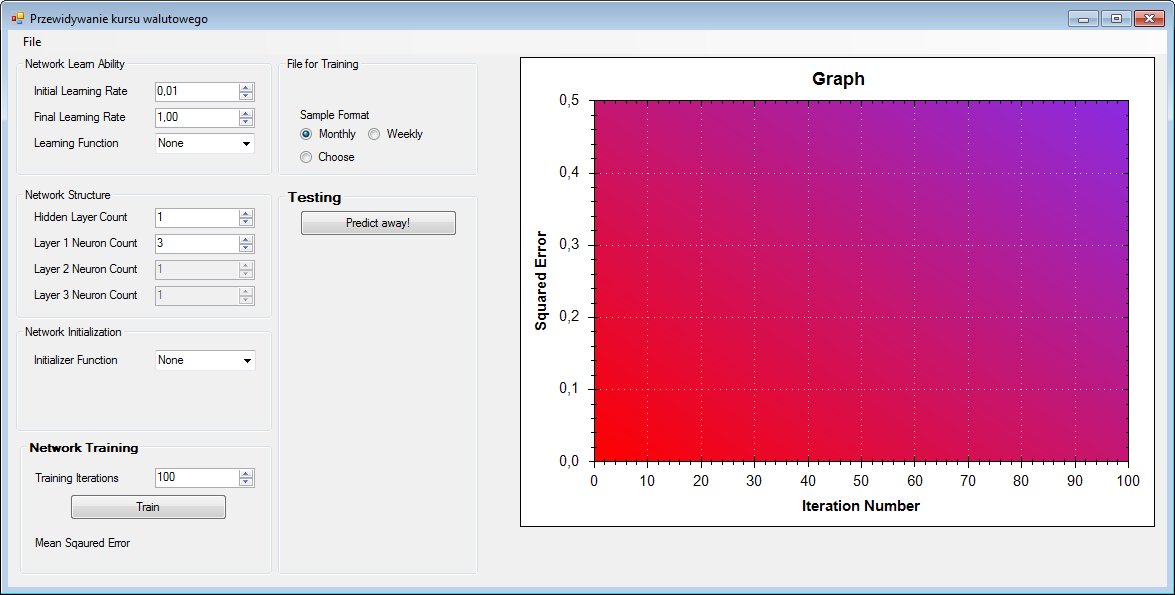
\includegraphics[width=0.90\textwidth]{./img/GUI}
				\caption{Interfejs po uruchomieniu programu}
			\end{figure}
			Przed przystąpieniem do trenowania sieci można są skonfigurować:
			\subsection{Struktura sieci}
				\begin{figure}[h!]
					\centering
					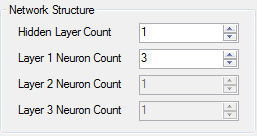
\includegraphics[width=0.40\textwidth]{./img/GUI_network_structure}
					\caption{Panel do konfiguracji struktury sieci z domyślnymi wartościami}
				\end{figure}
				W tym panelu definiuje się budowę wewnętrzną sieci neuronowej - liczbę warstw pośrednich oraz liczbę neuronów w każdej z warstw. Maksymalnie można utworzyć 3 warstwy z minimum 1 neuronem. W zależności od wartości w polu \emph{Hidden Layer Count}, odpowiednie pola \emph{Layer Neuron Count} są dostępne lub nie.
			\newpage
			\subsection{Zdolność nauki}
				\begin{figure}[h!]
					\centering
					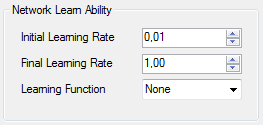
\includegraphics[width=0.40\textwidth]{./img/GUI_initial_learning}
					\caption{Panel do konfiguracji zdolności nauki z domyślnymi wartościami}
				\end{figure}
				Ten panel znajduje się w górnym lewym rogu interfejsu. Umożliwia konfigurację trzech parametrów:
				\begin{itemize}
					\item \emph{Initial Learning Rate} - wartość startowa zdolności nauki, z nią uruchamiany jest trening sieci.
					\item \emph{Final Learning Rate} - wartość zdolności nauki, którą sieć będzie miała, gdy trening się skończy.
					\item \emph{Learning Function} - specjalizowana funkcja, jakiej sieć backpropagacji będzie wykorzystywać do nauki. Są cztery możliwości:
					\begin{itemize}
						\item \emph{None} - standardowa funkcja
						\item \emph{Expotential} - funkcja eksponencjalna
						\item \emph{Hyperbolic} - funkcja hiperboliczna
						\item \emph{Linear} - funkcja liniowa
					\end{itemize}
				\end{itemize}
			\subsection{Inicjalizacja funkcji}
				\begin{figure}[h!]
					\centering
					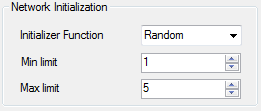
\includegraphics[width=0.40\textwidth]{./img/GUI_network_initialization}
					\caption{Panel do konfiguracji inicjalizacji sieci z przykładowymi ustawieniami}
				\end{figure}
				W tej części (lewa strona interfejsu) można ustawić inicjalizację sieci, czyli początkową wartość wag neuronów we wszystkich warstwach. Istnieje cześć możliwości:
				\begin{itemize}
					\item \emph{None} - wartości domyślne.
					\item \emph{Constant} - wskazana wartość stała.
					\item \emph{NgyuenWidrow} - sparametryzowana funkcja\textit{ NGuyen Widrow}.
					\item \emph{NormalizedRandom} - znormalizowana wartość losowa.
					\item \emph{Random} - wartość losowa ze wskazanego zakresu.
					\item \emph{Zero} - funkcja typu Zero (wszystkie wartości są zbliżone do zera).
				\end{itemize}
			\newpage
			\subsection{Analiza plików}
				\begin{figure}[h!]
					\centering
					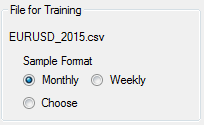
\includegraphics[width=0.40\textwidth]{./img/GUI_files}
					\caption{Panel z wczytanym plikiem i sposobem podziału}
				\end{figure}
				Ten panel znajduje się w górnej środkowej części interfejsu. Umożliwia pogląd załadowanego pliku do treningu sieci (tutaj \textit{EURUSD\_2015.csv}) oraz sposób w jaki dane będą grupowane:
				\begin{itemize}
					\item \emph{Monthly} - co miesiąc.
					\item \emph{Weekly} - co tydzień.
					\item \emph{Choose} - wg wskazanej przez użytkownika liczby dni.
				\end{itemize}
			\subsection{Trening sieci}
				\begin{figure}[h!]
					\centering
					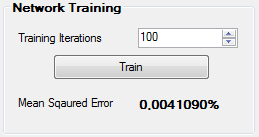
\includegraphics[width=0.40\textwidth]{./img/GUI_network_training}
					\caption{Przykładowy wynik trenowania sieci po 100 iteracjach}
				\end{figure}
				Ten panel znajduje się w dolnym prawym rogu. Wymaga od użytkownika wprowadzania liczby iteracji treningowych, jakie wykona sieć (domyślnie jest to wartość 100). Po wciśnięciu przycisku \emph{Train} sieć rozpocznie swój trening. Gdy zostanie on zakończony, na dole pojawia się \emph{Mean Sqaured Error} (średni kwadratowy błąd) sieci w procentach. Oznacza on jakie wg obliczeń jest prawdopodobieństwo błędu sieci, czyli złego przewidzenia linii trendu kursu waluty.\\
				Program poświęca 70\% próbek (zaokrąglonych w górę) do testów.
			\newpage
			\subsection{Trening sieci}
				\begin{figure}[h!]
					\centering
					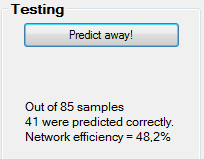
\includegraphics[width=0.30\textwidth]{./img/GUI_testing}
					\caption{Przykładowy wynik testowania sieci}
				\end{figure}
				Na środku interfejsu znajduje się przycisk \emph{Predict away!}. Gdy sieć została wytrenowana i skonfigurowana, jego wciśnięcie powoduje uruchomienie testowania sieci i zmierzenie jej efektywności. Po wykonaniu testów informacje zostaną wyświetlone w tym samym panelu.\\ Program poświęca 30\% próbek w celu zbadania jakości działania sieci.
			\subsection{Graf błędu}
				\begin{figure}[h!]
					\centering
					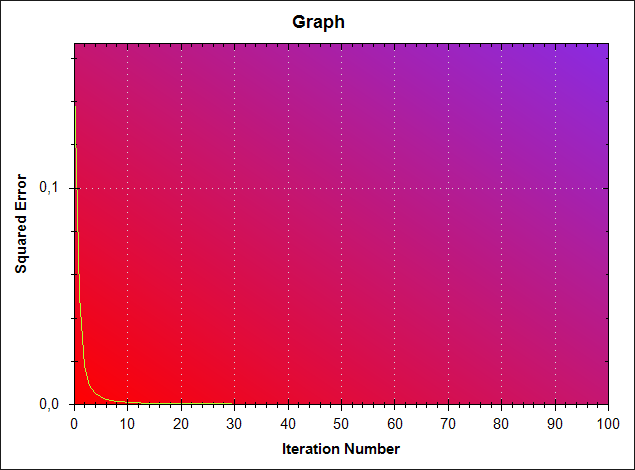
\includegraphics[width=0.85\textwidth]{./img/GUI_graph}
					\caption{Przykładowy przebieg nauki sieci}
				\end{figure}
				W czasie treningu sieci jest generowany graf zależności jakości sieci od liczby iteracji. Przedstawia on jak prawdopodobieństwo błędu zmieniało się wraz z kolejnymi iteracjami. Można powiedzieć, że obrazuje on, w jaki sposób sieć się uczy.\\
				Maksymalną wartością na osi poziomej jest liczba iteracji, z kolei na osi pionowej jest to maksymalny średni błąd kwadratowy (wyliczany dynamicznie w trakcie działania programu).
			
	
	
	
\end{document}